\documentclass[%
reprint,
%superscriptaddress,
%groupedaddress,
%unsortedaddress,
%runinaddress,
%frontmatterverbose, 
%preprint,
%preprintnumbers,
%nofootinbib,
%nobibnotes,
%bibnotes,
amsmath,amssymb,
aps,
%pra,
%prb,
%rmp,
%prstab,
%prstper,
%floatfix,
]{revtex4-2}
\usepackage{multirow}
\usepackage{graphicx}% Include figure files
\usepackage{dcolumn}% Align table columns on decimal point
\usepackage{bm}% bold math
%\usepackage{hyperref}% add hypertext capabilities
%\usepackage[mathlines]{lineno}% Enable numbering of text and display math
%\linenumbers\relax % Commence numbering lines

%\usepackage[showframe,%Uncomment any one of the following lines to test 
%%scale=0.7, marginratio={1:1, 2:3}, ignoreall,% default settings
%%text={7in,10in},centering,
%%margin=1.5in,
%%total={6.5in,8.75in}, top=1.2in, left=0.9in, includefoot,
%%height=10in,a5paper,hmargin={3cm,0.8in},
%]{geometry}
\usepackage[utf8x]{inputenc} % Включаем поддержку UTF8  
\usepackage[russian]{babel}  % Включаем пакет для поддержки русского языка 
\usepackage[normalem]{ulem}  % для зачекивания текста

\usepackage[noend]{algorithmic}
\def\algorithmicrequire{\textbf{Вход:}}
\def\algorithmicensure{\textbf{Выход:}}
\def\algorithmicif{\textbf{если}}
\def\algorithmicthen{\textbf{то}}
\def\algorithmicelse{\textbf{иначе}}
\def\algorithmicelsif{\textbf{иначе если}}
\def\algorithmicfor{\textbf{для}}
\def\algorithmicforall{\textbf{для всех}}
\def\algorithmicdo{}
\def\algorithmicwhile{\textbf{пока}}
\def\algorithmicrepeat{\textbf{повторять}}
\def\algorithmicuntil{\textbf{пока}}
\def\algorithmicloop{\textbf{цикл}}
% переопределение стиля комментариев
\def\algorithmiccomment#1{\quad// {\sl #1}}

\usepackage{caption}
\usepackage{subcaption}
\usepackage{multirow}
\usepackage[table,xcdraw]{xcolor}

\begin{document}
	
	
	
	\title{Лабораторная работа 5.1. Измерение ослабления потока $\gamma$ лучей в веществе и определение их энергий}% Force line breaks with \\
	
	
	
	\author{Батарин Егор Владиславович}
	\affiliation{%
		Студент 3 курса ФРТК\\
	}%
	
	\collaboration{Московский физико-технический институт}%\noaffiliation
	
	\date{15 ноября 2021 г.}% It is always \today, today,
	%  but any date may be explicitly specified
	
	
	\begin{abstract}
		\textbf{Цель работы:} используя сцинтилляционный счетчик, измерить линейные коэффициенты ослабления потока $\gamma$ лучей в свинце, железе и алюминии; по их величине определить энергию $\gamma$ квантов.
		\begin{description}
			\item[Оборудование]
			свинцовый коллиматор, источник лучей, свинцовый контейнер с коллиматорным каналом, набор поглотителей, сцинтиллятор (кристалл NaI), формирователь-выпрямитель.
		\end{description}
	\end{abstract}
	
	%\keywords{Suggested keywords}%Use showkeys class option if keyword
	%display desired
	\maketitle
	
	%\tableofcontents
	
	\section{Теоретическая часть.}
	
	При прохождении пучка гамма-квантов через вещество, энергия данного пучка уменьшается по экспоненциальному закону:
	\[I = I_{0} e^{-\mu l}\].
	Уменьшение связано с тремя главными эффектами: фотоэлектрическим поглощением, комптоновским рассеянием и образованием электрон-позитронных пар.
	
	Для определение коэффициента $\mu$ будем использовать следующие рассуждения: при выбывании из пучка $dN$ гамма-квантов на пути $dl$, имеем очевидное соотношение:
	\[-dN = \mu N dl\]
	
	Интегрируя данное уравнение от нулевой толщины до заданной, получаем:
	
	\[N = N_{0} e^{-\gamma l}\]
	
	И тогда для коэффициента $\mu$ имеем:
	
	\[\mu = \frac{1}{l} \ln{\frac{N_{0}}{N}}\]
		
		
	\section{Результаты эксперимента}
	
	\subsection{Результаты измерений}
	
	\begin{table}[]
		\begin{tabular}{|l|l|l|l|l|}
			\hline
			Фон (без образца)          &                     &                  &                  &       \\ \hline
			235835                     &                     &                  &                  &       \\ \hline
			241980                     &                     &                  &                  &       \\ \hline
			242480                     &                     &                  &                  &       \\ \hline
			241583                     &                     &                  &                  &       \\ \hline
			243039                     &                     &                  &                  &       \\ \hline
			239366                     &                     &                  &                  &       \\ \hline
			239191                     &                     &                  &                  &       \\ \hline
			239316                     &                     &                  &                  &       \\ \hline
			Фон (с заглушкой)          & Среднее             & Отклонение       & Погрешность, \%  &       \\ \hline
			141                        & 144.75              & 5.56027577253743 & 3.84129587049218 &       \\ \hline
			142                        &                     &                  &                  &       \\ \hline
			143                        &                     &                  &                  &       \\ \hline
			153                        &                     &                  &                  &       \\ \hline
			Fe (данные с вычетом фона) & Толщина образца, см &                  &                  &       \\ \hline
			& 1                   & 2                & 3                & 4     \\ \hline
			& 114675              & 57198            & 29382            & 15050 \\ \hline
			& 114164              & 57049            & 29591            & 15114 \\ \hline
			& 114189              & 56799            & 29627            & 15305 \\ \hline
			& 113795              & 56910            & 29451            & 15168 \\ \hline
			& 114237              & 57011            & 29445            & 15235 \\ \hline
			&                     & 56857            & 29414            & 14956 \\ \hline
			&                     & 56810            &                  & 15121 \\ \hline
			&                     &                  &                  & 15096 \\ \hline
			Al (данные с вычетом фона) & Толщина образца, см &                  &                  &       \\ \hline
			& 2                   & 4                & 6                & 8     \\ \hline
			& 136560              & 79517            & 48126            & 29760 \\ \hline
			& 136447              & 79032            & 48059            & 29628 \\ \hline
			& 137340              & 78918            & 48427            & 29879 \\ \hline
			& 136922              & 79229            & 48373            & 29796 \\ \hline
			& 137297              & 79483            & 48090            & 29828 \\ \hline
			& 137647              & 79555            & 48367            & 29848 \\ \hline
			& 136994              & 79118            & 48369            & 29863 \\ \hline
			& 136888              &                  & 48399            & 29803 \\ \hline
			& 136990              &                  & 48346            &       \\ \hline
			& 137210              &                  & 48186            &       \\ \hline
			& Толщина образца, см &                  &                  &       \\ \hline
			Pb (данные с вычетом фона) & 0.45                & 0.9              & 1.35             & 1.8   \\ \hline
			& 115032              & 57292            & 30168            & 17129 \\ \hline
			& 115356              & 56777            & 30121            & 17041 \\ \hline
			& 114355              & 57026            & 30304            & 17100 \\ \hline
			& 115241              & 57278            & 30127            & 17117 \\ \hline
			& 115265              & 57319            & 30367            & 17185 \\ \hline
			& 115461              & 57120            & 30161            & 17195 \\ \hline
			& 114481              & 57327            & 30163            & 17087 \\ \hline
			& 115281              & 57401            & 30426            & 17082 \\ \hline
			& 115036              & 57114            & 30232            &    \\ \hline
		\end{tabular}
	\end{table}




	Все результаты измерений сведены в таблицу. 
	
	Оценивая погрешность, было учтено, что в суммарную погрешность вычисления коэффициента входит погрешность вычисления толщины образца (0.005 сантиметров у штангенциркуля) и пошрешность вычисления количество гамма-квантов, вылетающих из щели без образца. Погрешность измерения количества прошедших квантов была сведена к минимуму и в расчете погрешности она несравнимо мала с указанными выше погрешностями.
	
	Итого получаем: 
	
	$\mu_{Fe} = 0.666 \pm 0.005 \text{ см}^{-1}$
	
	
	 $\mu_{Al} = 0.244 \pm 0.005 \text{ см}^{-1}$
	 
	 
	  $\mu_{Pb} = 1.309 \pm 0.005 \text{ см}^{-1}$
	  
	  
	Сравнивая со значениями коэффициента ослабления из таблицы, получаем следующие значения энергии гамма-квантов:
	
	 $E_{\gamma Fe} = 0.5\text{МэВ}$
	
	$E_{\gamma AL} = 0.5\text{МэВ}$
	
	$E_{\gamma Pb} = 0.6\text{МэВ}$
	
	Немного не совпало значение для свинца.
	  
	  
	
	
	
	\section{Заключение}
	
	В результате данной работы были вычислены коэффициенты ослабления для трех веществ: железа, алюминия и свинца, а вычислены энергии гамма-квантов, использующихся в работе.
	
	
	\begin{figure}[]
		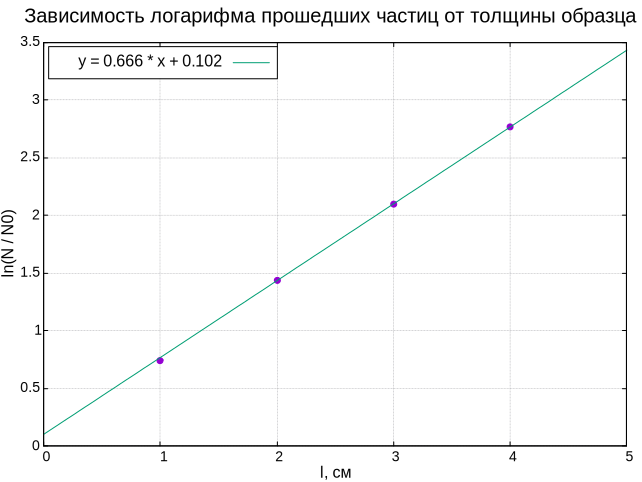
\includegraphics[width=\linewidth]{ratio-length-fe.pdf}
	\end{figure}
	
	\begin{figure}[]
		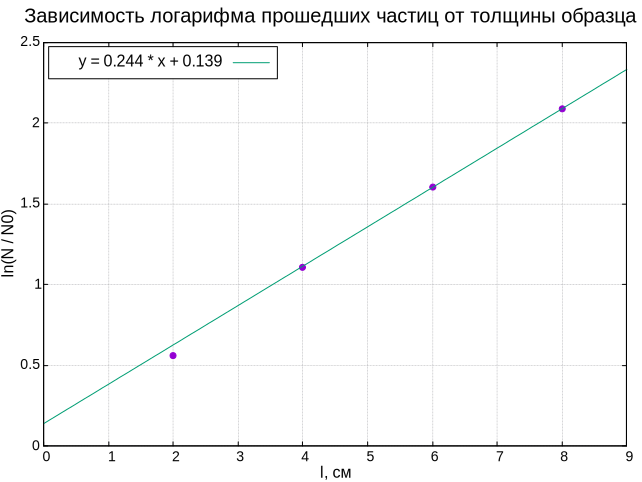
\includegraphics[width=\linewidth]{ratio-length-al.pdf}
	\end{figure}
	
	\begin{figure}[]
		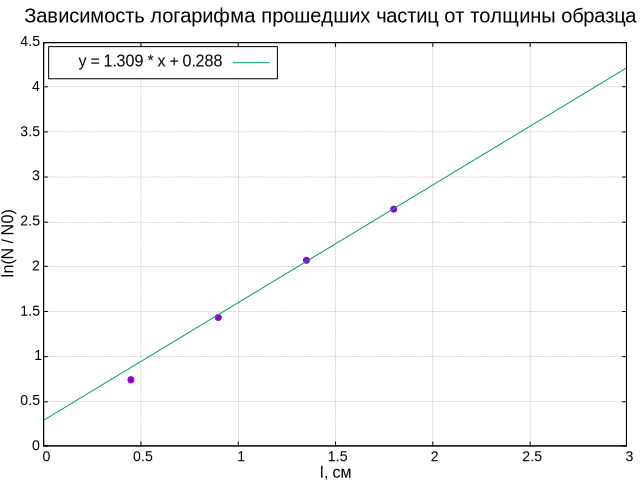
\includegraphics[width=\linewidth]{ratio-length-pb.pdf}
	\end{figure}
	
	
	
\end{document}